% Template LaTeX file for DAFx-08 papers % (fold)
%
% To generate the correct references using BibTeX, run
%     latex, bibtex, latex, latex
% modified...
% - from DAFx-00 to DAFx-02 by Florian Keiler, 2002-07-08
% - from DAFx-02 to DAFx-03 by Gianpaolo Evangelista
% - from DAFx-05 to DAFx-06 by Vincent Verfaille, 2006-02-05
% - from DAFx-06 to DAFx-07 by Vincent Verfaille, 2007-01-05
%                          and Sylvain Marchand, 2007-01-31
% - from DAFx-07 to DAFx-08 by Henri Penttinen, 2007-12-12
%                          and Jyri Pakarinen 2008-01-28
%
% Template with hyper-references (links) active after conversion to pdf
% (with the distiller) or if compiled with pdflatex.
%
% 20060205: added package 'hypcap' to correct hyperlinks to figures and tables
%                      use of \papertitle and \paperauthorA, etc for same title in PdF and Metadata
%
% 1) Please compile using latex or pdflatex.
% 2) If using pdflatex, you need your figures in a file format other than eps! e.g. png or jpg is working
% 3) Please use "paperftitle" and "pdfauthor" definitions below


%%%%%%%%%%%%%%%%%%%%%%%%%%%%%%%%%%%%%%%%%%%%%%%%%%%%%%%%%%%%%%%%%%%%%
%%%%%%%%%%%%%%%%%%%%%%%%%%%%%%%%%%%%%%%%%%%%%%%%%%%%%%%%%%%%%%%%%%%%%
%%%%%%%%%%%%%%%%%%%%%%%%%%%%%%%%%%%%%%%%%%%%%%%%%%%%%%%%%%%%%%%%%%%%%
% 
% TTBlue Notes / Paper
% from conversation with Dave over coffee at Pre en Bulle in Albi
% 20 June 2008
% 
% Allows for:
% * programmatic creation of user interfaces
% * adaptive wrappers for various plug-in architectures (VST, AU, Max/MSP, SuperCollider)
% * dynamic, self-modifying networks of components 
% 
% Dynamic re-configuration of the signal networks and control structures means that TTBlue can be run on a web server and the signal chain defined (or re-defined) in real time on a web client using a GUI (such as a web browser or iPhone) or SMS.
% 
% One application of this is an installation or sculptural art work where you could tweak the behavior by sending it SMS messages using a phone.



%%%%%%%%%%%%%%%%%%%%%%%%%%%%%%%%%%%%%%%%%%%%%%%%%%%%%%%%%%%%%%%%%%%%%
%%%%%%%%%%%%%%%%%%%%%%%%%%%%%%%%%%%%%%%%%%%%%%%%%%%%%%%%%%%%%%%%%%%%%
%%%%%%%%%%%%%%%%%%%%%%%%%%%%%%%%%%%%%%%%%%%%%%%%%%%%%%%%%%%%%%%%%%%%%




%------------------------------------------------------------------------------------------
%  !  !  !  !  !  !  !  !  !  !  !  ! user defined variables  !  !  !  !  !  !  !  !  !  !  !  !  !  !
% Please use these commands to define title and author of the paper:
\def\papertitle{The Jamoma Audio Graph Layer}
\def\paperauthorA{Timothy Place}
\def\paperauthorB{Trond Lossius}
\def\paperauthorC{Nils Peters}


%------------------------------------------------------------------------------------------
\documentclass[twoside,a4paper]{article}
\usepackage{dafx_08}
\usepackage{amsmath,amssymb,amsfonts,amsthm}
\usepackage{subfigure,color}
\usepackage{euscript}
\usepackage[latin1]{inputenc}
\usepackage[T1]{fontenc}    
%% %%%% for source code listing %%%%%%%%%%%
\usepackage{listings}						% required for source code listings

% Enables multi-line comments:
\usepackage{verbatim} 
\lstset{language=c++}
\lstset{basicstyle=\footnotesize\ttfamily}
\lstset{commentstyle=\color{commentcolor}}
\lstset{tabsize=2}  
\lstset{gobble=2}							% eat the first tab in block listings
\lstset{aboveskip=\bigskipamount}			% amount of space above a block listing
\lstset{belowskip=\bigskipamount}			% ... 
\newenvironment{packed_item}{
\begin{itemize}
  \setlength{\itemsep}{1pt}
  \setlength{\parskip}{0pt}
  \setlength{\parsep}{0pt}
}{\end{itemize}}
%%
\setcounter{page}{1}
\ninept

\usepackage{times}
% Saves a lot of ouptut space in PdF... after conversion with the distiller
% Delete if you cannot get PS fonts working on your system.

% pdf-tex settings: detect automatically if run by latex or pdflatex
%\newif\ifpdf
%\ifx\pdfoutput\relax
%\else
%   \ifcase\pdfoutput
%      \pdffalse
%   \else
%      \pdftrue
%\fi
%\ifpdf % compiling with pdflatex
  \usepackage[pdftex,
    pdftitle={\papertitle},
    pdfauthor={\paperauthorA, \paperauthorB, \paperauthorC},
    colorlinks=true, % links are activated as colror boxes instead of color text
		linkcolor=black,
		urlcolor=black,
		citecolor=black,
    bookmarksnumbered, % use section numbers with bookmarks
    pdfstartview=XYZ % start with zoom=100% instead of full screen; especially useful if working with a big screen :-)
  ]{hyperref}
  \pdfcompresslevel=9
  \usepackage[pdftex]{graphicx}
  \usepackage[figure,table]{hypcap}
%\else % compiling with latex
%  \usepackage[dvips]{epsfig,graphicx}
%  \usepackage[dvips,
%    colorlinks=false, % no color links
%    bookmarksnumbered, % use section numbers with bookmarks
%    pdfstartview=XYZ % start with zoom=100% instead of full screen
%  ]{hyperref}
%  % hyperrefs are active in the pdf file after conversion
%  \usepackage[figure,table]{hypcap}
%\fi

\title{\papertitle}

%-------------SINGLE-AUTHOR HEADER STARTS (uncomment below if your paper has a single author)-----------------------
%\affiliation{\paperauthorA}    % This command replaces \name{The DAFx Crew}
%{\href{http://www.acoustics.hut.fi/dafx08/}{Dept. of Signal Processing and Acoustics,} \\ Helsinki University of Technology, TKK \\ Espoo, Finland\\
%{\tt \href{mailto:dafx-08@acoustics.hut.fi}{dafx-08@acoustics.hut.fi}}}
%-----------------------------------SINGLE-AUTHOR HEADER ENDS------------------------------------------------------

%---------------TWO-AUTHOR HEADER STARTS (uncomment below if your paper has two authors)-----------------------
%\twoaffiliations{\paperauthorA, \sthanks{This work was supported by the XYZ Foundation}}
%{\href{
%http://www.acoustics.hut.fi/dafx08/}{Dept. of Signal Processing and Acoustics,} \\ Helsinki University of Technology, TKK \\ Espoo, Finland\\
%{\tt \href{mailto:dafx-08@acoustics.hut.fi}{dafx-08@acoustics.hut.fi}}
%}
%{\paperauthorB,\sthanks{This guy is a very good fellow}}
%{\href{http://www.acoustics.hut.fi/dafx08/}{Reading Group, Dept.~of Reading Sciences} \\ Univ.~of Universe, Sun \\ {\tt \href{mailto:dafx-08@acoustics.hut.fi}{dafx-08@acoustics.hut.fi}}
%}
%-------------------------------------TWO-AUTHOR HEADER ENDS------------------------------------------------------

%---------------THREE-AUTHOR HEADER STARTS (uncomment below if your paper has three authors)-----------------------
\threeaffiliations{\paperauthorA}
{\href{http://74objects.com}{74 Objects LLC,} \\ Kansas City, Missouri, USA\\
{\tt \href{mailto:tim@74objects.com}{tim@74objects.com}}
}
{\paperauthorB}
{\href{http://www.bek.no/}{BEK - Bergen Center for Electronic Arts} \\ Bergen, Norway\\ {\tt \href{mailto:trond.lossius@bek.no}{trond.lossius@bek.no}}
}
{\paperauthorC}%,\sthanks{Is still sore from ice climbing}
{\href{http://www.music.mcgill.ca/musictech/}{McGill University, CIRMMT} \\ Montreal, Quebec, Canada\\{\tt \href{mailto:nils.peters@mcgill.ca}{nils.peters@mcgill.ca}}     %CIRMMT - Centre for Interdisciplinary Research in Music Media and Technology\\
}
%-------------------------------------THREE-AUTHOR HEADER ENDS------------------------------------------------------

% (end)

\hyphenation{a-syn-chro-nous ja-mo-ma}

\begin{document}
% more pdf-tex settings:
%\ifpdf % used graphic file format for pdflatex
  \DeclareGraphicsExtensions{.png,.jpg,.pdf}
%\else  % used graphic file format for latex
%  \DeclareGraphicsExtensions{.eps}
%\fi

\maketitle
\sloppy


%%%%%%%%%%%%%%%%%%%%%%%%%%%%%%%%%%%%%%%%%%%%%%%%%%%%%%%%%%%%%%%%%%%%%
%
\begin{abstract} % (fold)
%
%%%%%%%%%%%%%%%%%%%%%%%%%%%%%%%%%%%%%%%%%%%%%%%%%%%%%%%%%%%%%%%%%%%%%
%
Jamoma Audio Graph is a framework for creating graph structures in which unit generators are connected together to process dynamic multi-channel audio in real-time.  
These graph structures are particularly well-suited to spatial audio contexts demanding large numbers of audio channels, such as Higher Order Ambisonics, Wave Field Synthesis and microphone arrays for beamforming.
% TODO: I'm not convinced that we currently should mention WFS, as we don't have support for it anywhere in Jamoma so far.
This framework forms part of the Jamoma layered architecture for interactive systems, with current implementations of Jamoma Audio Graph targeting the Max/MSP, PureData, Ruby, and AudioUnit environments.

\end{abstract} % (end)




%%%%%%%%%%%%%%%%%%%%%%%%%%%%%%%%%%%%%%%%%%%%%%%%%%%%%%%%%%%%%%%%%%%%%
%
\section{Introduction} % (fold)
%
%%%%%%%%%%%%%%%%%%%%%%%%%%%%%%%%%%%%%%%%%%%%%%%%%%%%%%%%%%%%%%%%%%%%%

\label{sec:intro}
% TODO: I feel that we don't really say WHY we develop this framework. We develop this because ..........   
%		Can we answer this in the Requirements section?  [TAP]

Many frameworks, toolkits, and environments for real-time audio fuse the issues of creating unit generators with creating graph structures\footnote{Wikipedia defines this by saying ``a graph is an abstract representation of a set of objects where some pairs of the objects are connected by links''. \url{http://en.wikipedia.org/wiki/Graph_(mathematics)}} that process audio through those unit generators.
% TODO: Could we come up with a better and more permanent reference for this definition than Wikipedia? What do Wikipedia itself reference?
% CHANGED: I moved the footnote one word to the right (after structure) as that seems to work better with the text flow - TL
Alternatively, the Jamoma Platform implements a clear separation of concerns, structured in a layered architecture of several frameworks \cite{Place:2010}.
Six frameworks currently comprise the Jamoma Platform, providing a comprehensive infrastructure for creating computer music systems. 
These frameworks are: Jamoma Foundation, Jamoma Graphics, Jamoma Modular, Jamoma DSP, Jamoma Graph and Jamoma Audio Graph (see Figure~\ref{fig:layers}).

Jamoma Foundation provides low-level support, base classes, and communication systems; Jamoma Graphics provides screen graphics; Jamoma Modular provides a structured approach to development and control of modules in the graphical media environment Max \cite{Place:2006} and Jamoma DSP specializes the Foundation classes to provide a framework for creating a library of unit generators. 
Jamoma Graph networks Jamoma Foundation based objects into graph structures, providing a basic asynchronous processing model for objects (nodes) in the graph structure. 
Jamoma Audio Graph (JAG), the focus of this paper, is an open source C++ framework that extends and specializes the Jamoma Graph layer.  It provides the ability to create and network Jamoma DSP objects into dynamic graph structures for synchronous audio processing\footnote{Licensing for all layers of the Jamoma Platform are provided under the terms of the GNU LGPL}.  


\begin{figure}[htbp]
\centerline{\framebox{
	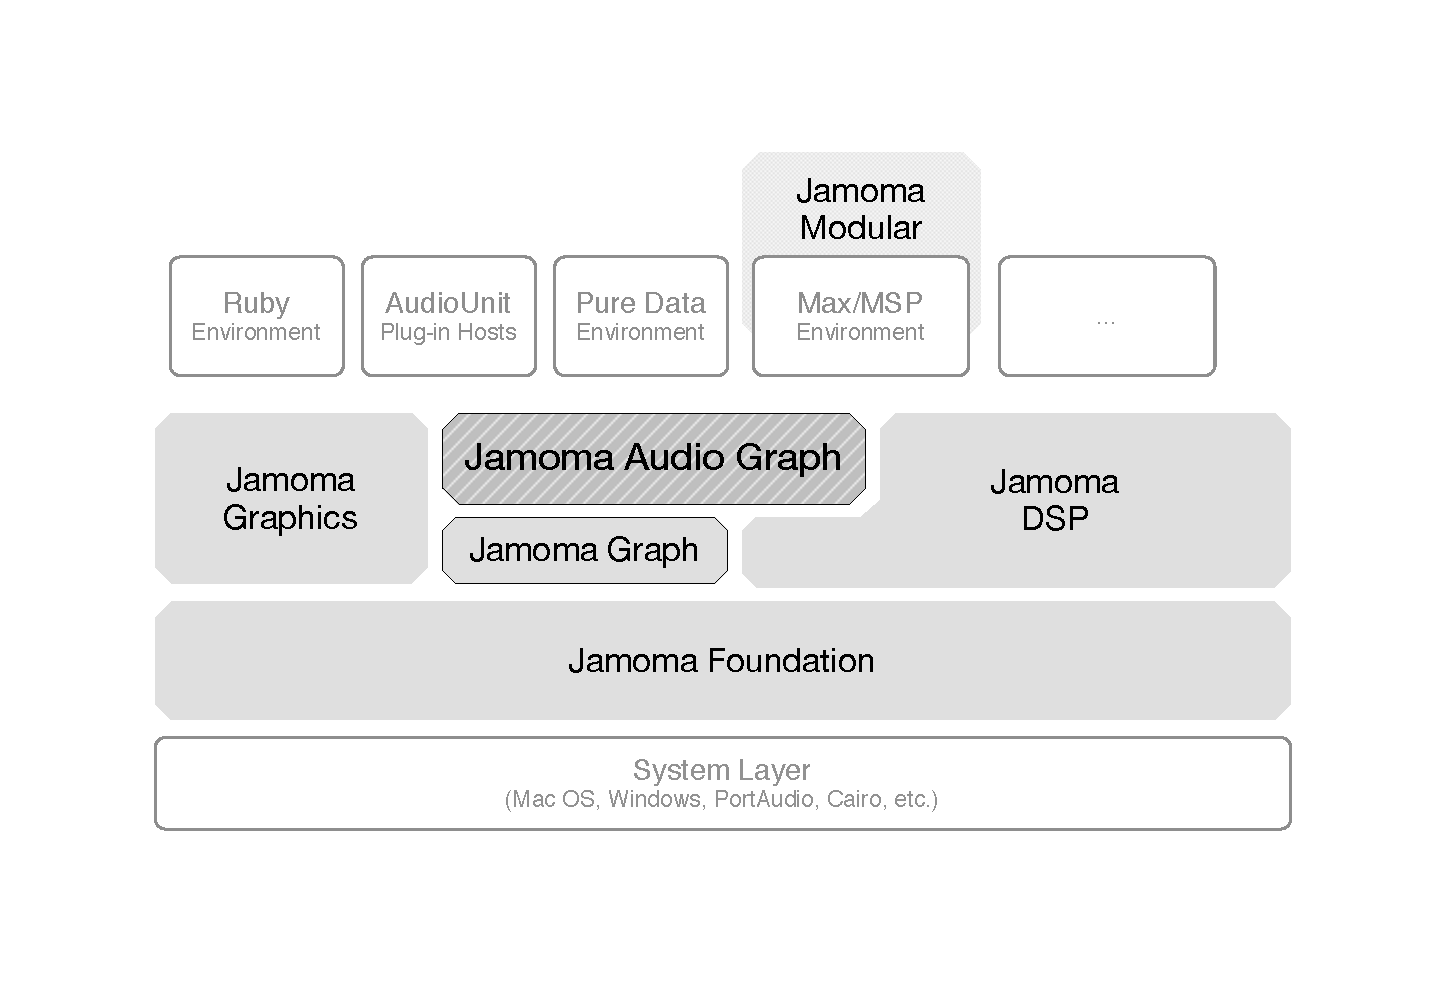
\includegraphics[width=0.95\columnwidth]{layers-multicore}}}
\caption{The Jamoma Platform as Layered Architecture.}
\label{fig:layers}
\end{figure}


\subsection{Requirements}

Through years of accumulated collective experience in a myriad of contexts for realtime multi-channel audio work, we found a number of practical needs were still unmet by readily available environments.  We believe the following necessities are required not only to ease usability concerns in some environments, but also to open new avenues of creation, exchange, performance, and research in digital audio effects.

\begin{packed_item}
	\item{Connections between objects must be capable of delivering multiple channels of audio}
	\item{Support for audio signals with multiple sample rates and vector sizes simultaneously within a graph}
	\item{Audio signal sample rate, vector size, and number of channels must be dynamic (able to be changed in realtime)}
	\item{Dynamic modification of an audio graph at runtime (Live coding/Live patching)}    
	\item{Ability to transport representations of an audio graph between different programming languages}
	\item{Support for multi-threaded parallel audio processing}
	\item{Liberal licensing for both open source and commercial use}
	\item{Cross-platform}
	%\item{Sending information about the channel's audio content as meta data}  
	% CHANGED: we aren't really doing this last thing right now [TAP]
\end{packed_item}	

In order to best meet these requirements, Jamoma Audio Graph relies on a \emph{pull} pattern (see Section~\ref{sec:pull}) and is designed to be independent from the host environment's DSP scheduler.
An additional design decision is the use of a ``peer object model" which abstracts the implementation and execution of the graph from any particular environment or platform.  
This allows for the Jamoma Audio Graph layer to be readily implemented for any number of environments.
To date the authors have created implementations for Max, PureData, Audio Units, and Ruby.
% NP: the term peer object model is unclear to me -- maybe the whole peer-object thing should go into the background

% TODO For list of requirements:  Decoupling Graph and Unit Generator

%- presenting distinguishing between graph and units
%    - what is a graph and a unit?
%
%- application for Jamoma Audio Graph
%    - e.g. up/downmixing; encoding/decoding 

% (end)




%%%%%%%%%%%%%%%%%%%%%%%%%%%%%%%%%%%%%%%%%%%%%%%%%%%%%%%%%%%%%%%%%%%%%
%
\section{Background} % (fold)
%
%%%%%%%%%%%%%%%%%%%%%%%%%%%%%%%%%%%%%%%%%%%%%%%%%%%%%%%%%%%%%%%%%%%%%


% TODO: begin with the historical background -- the difficulty of patching multi-channel/ambisonic object networks in MSP, etc. etc. etc.

\subsection{Decoupling Graph and Unit Generator} % (fold)

The Jamoma DSP framework for creating unit generators does not define the way in which one must produce signal processing topographies.  
Instead, the process of creating objects and connecting them are envisioned and implemented orthogonally and the graph is created using a separate framework: Jamoma Audio Graph.  
Thanks to this decoupling of Jamoma DSP and Jamoma Audio Graph we are able to create and use Jamoma DSP unit generators with a number of different graph structures.  
Jamoma Audio Graph is one graph structure that a developer may choose to employ.

Max/MSP, Pd, SuperCollider, Csound, Bidule, AudioMulch, Reaktor and Reason all have have unit generators, but the unit generators can only be used within the particular environment. 
The unit generators have a proprietary format and thus no interchangeability.  Likewise, the graph structure is proprietary. 
While SDKs are available for some of these environments, for others no SDK exists and the systems are closed. 
Ability to host Audio Units and VST may extend these environments, but with limitations.

% (end)


\subsection{Audio Graph Structures} % (fold)

A graph structure is an abstract structure where paths are created between nodes (objects) in a set.
The paths between these nodes then define the data-flow of the graph.
Graph structures for audio signal processing employ several patterns and idioms to achieve a balance of efficiency, flexibility, and real-time capability.

Environments for real-time processing typically need to address concerns in both synchronous and asynchronous contexts.  
Asynchronous communication is required for handling MIDI, mouse-clicks and other user interactions, the receipt of Open Sound Control messages from a network, and often for driving attributes from audio sequencer automations.
Conversely, realtime processing of audio streams must be handled synchronously.  
Most environments, such as CLAM  \cite{Amatraian:2007}, deal with these two types of graphs as separate from each other.  
In the Jamoma Platform this is also the case, where Jamoma Audio Graph comprises the synchronous audio graph concerns, and Jamoma Graph implements asynchronous message passing.

% TODO: Is the synchronous/asynchronous a tad to specific here and we are rather thinking in terms of audio rate and control rate? In Csound e.g. we are talking k-rate and a-rate. k-rate is processed at a lower sample rate than a-rate, but to the best of my knowledge is still synced to the audio processing. - TL
% NO: control-rate is a simply a sub-rate of the audio-rate that runs more slowly, e.g. for ramps.  Asynchronous is like MIDI where there is no rate at all: messages just come in whenever a key is pressed or a slider moved [TAP]

To reduce the computational overhead of making synchronous calls through the graph for every sample, most systems employ the notion of \emph{frame processing}.  
The Jamoma Audio Graph processes blocks of samples at once rather than a single sample at a time.  
These blocks of samples are passed using a Jamoma DSP class that represents audio signals.  This class bundles vectors of audio for multiple channels together with an interface for accessing the signal's data and metadata.
% TODO: From a mathematical viewpoint I am not convinced that it is correct to use the word "vector" for multi-channel frames, as these "vectors" really are 2-dimensional and hence matrixes: M samples x N channels. See e.g. http://mathworld.wolfram.com/Vector.html for a definition of "vector" - TL
% I believe that we aren't really allocating a matrix though, we are actually working on this as an array of vectors [TAP]

% (end)


\subsection{Push vs. Pull} \label{sec:pull} % (fold)

When visualizing a signal processing graph, it is common to represent the flow of audio from top-to-bottom or left-to-right.  
Under the hood, the processing may be implemented in this top-to-bottom flow as well.  
Audio at the top of the graph `pushes' down through each subsequent object in the chain until it reaches the bottom.

Alternatively, audio processing may be driven from the bottom of the chain from a `terminal object' or `sink'.  
This strategy for processing an audio graph, the `pull' method, is used by several environments including Apple's AUGraph and ChucK \cite{wang:2008}. 
AUGraph and ChucK are subject to certain limitations however: AUGraph does not permit ``fanning'' connections (many inlets connected to one outlet)\footnote{http://developer.apple.com/mac/library/documentation/General/\\Conceptual/SLGlobalGlossary/Glossary/Glossary.html} while ChucK is not multi-threaded.
% CHANGED: Added a line break in footnote to make it look better. - TL 2010-01-01

% (end)


\subsection{Multi-channel Processing} % (fold)

In many real-time audio patching environments, such as Max/MSP, Pd, Bidule or AudioMulch, audio objects are connected using mono signals. 
For multi-channel spatial processing the patch has to be tailored to the number of sources and speakers. 
If such programs are considered programming environments and the patch the program, a change in the number of sources or speakers requires a rewrite of the program, not just a change to one or more configuration parameters.

% TODO: do we need citations for Max, Pd, Bidule, and AudioMulch?
% Here's a resource on spatialisation in Pd:
% http://grh.mur.at/misc/PdSpatialization.tar.gz
% (end)

\subsubsection{CSound} % (fold)

In Csound multi-channel audio graph possibilities are extended somewhat through the introduction of the ``chn'' set of opcodes.
% Zak enables flexible routing from one instrument to another as instruments may be reconfigured in the score without requiring changes to the orchestra \cite{Mikelson:2000} and is used e.g. by the \texttt{vbapz} opcode for multi-channel vector-base amplitude panning.
The ``chn'' opcodes provide access to a global string-indexed software bus enabling communicating between a host application and the Csound engine, but can also be used for dynamic routing within Csound itself \cite{Yi:2006}.
Below is an example of a simple multi-channel filter implementation using named software busses to iterate through the channels:

% Note: This example was provided by √òyvind Brandsegg. The code have proper spacing when typeset.

\begin{lstlisting}
; multi-channel filter, event handler 
    instr 2 
    iNumC    = p4      ; number of channels 
    iCF      = p5      ; filter cutoff 
    ichnNum  = 0       ; init the channel number 
; makeEvent:
    ichnNum  = ichnNum + 1
    event_i  "i", 3, 0, p3, ichnNum, iCF
    if ichnNum < iNumC igoto makeEvent
    endin

; multi-channel filter, audio processing
    instr 3    
    instance = p4
    iCF      = p5
    Sname    sprintf   "Signal_%i", instance        
    a1       chnget    Sname
    a1       butterlp  a1, iCF
             chnset    a1, Sname
    endin
\end{lstlisting}  

% (end)

\subsubsection{SuperCollider} % (fold)

SuperCollider employs an elegant solution by representing signals containing multiple channels of audio as arrays. 
When an array of audio signals is given as input to a unit generator it causes multi-channel expansion: multiple copies of the unit generator are spawned to create an array of unit generators, each processing a different signal from the array of inputs.
In the following example a stereo signal containing white and pink noise is filtered:

\begin{lstlisting}
\ {
		\\ Create stereo signal as array:
		p = [WhiteNoise.ar, PinkNoise.ar];
		
		\\ Biquad filter applied to array of channels:
		SOS.ar(p, 1, -1.992, 0.986, 1.992, -0.993, 0.1);
\ }.play
\end{lstlisting}


\begin{comment}
	
NP: my research into multi-channel capabilities with SC\\
seems to be simple\\     
a) making a 3 channel  Sine Oscillator 

\begin{lstlisting}
{ Out.ar( 0, [ SinOsc.ar, SinOsc.ar, SinOsc.ar ] ) }.play;
\end{lstlisting}
b) making a 24 channel sine wave oscillator in SC:
\begin{lstlisting}
{ Out.ar( 0, SinOsc.ar.dup(24) ) }.play;
\end{lstlisting}  

for more complex multi-channel handling by a system called Multichannel Expansion, see \url{http://danielnouri.org/docs/SuperColliderHelp/Other%20Topics/MultiChannel.html}

\end{comment} 

% Trond investigationg SuperCollider:

\begin{comment}

% Example 1: Read stereo sound file, apply filter to both channels, and output:

(
b = Buffer.read(s, "/Users/lossius/Music/AIFF/VT Mandela_lyd/Lange/klokkerhav.aif");

{ 	var sig, rho, theta, b1, b2;

	theta = MouseX.kr(0.2pi, pi);
	rho = MouseY.kr(0.6, 0.99);
	b1 = 2.0 * rho * cos(theta);
	b2 = rho.squared.neg;

	sig = PlayBuf.ar(2, b, BufRateScale.kr(b), doneAction:2);
	
	// This is elegant, both channels are filtered with same coefficients:
	SOS.ar(sig, 1.0, 0.0, 0.0, b1, b2)

}.play
)
% Example 2: Pink noise => ambisonic encoding => encoded signal is filtered => ambisonic decoding => out

% ******************************************
% Ambisonics: 1 source, 4 speakers
% ******************************************

(
{
	var ambi, a, rho, theta, b1, b2;
	
	// Mouse stuff controlling filter
	theta = MouseX.kr(0.2pi, pi);
	rho = MouseY.kr(0.6, 0.99);
	b1 = 2.0 * rho * cos(theta);
	b2 = rho.squared.neg;
	
	// sources
	p = PinkNoise.ar;
	
	// B-format encode
	ambi = PanB2.ar(p, MouseX.kr(-1,1), 0.1); 

	// Now we do some weird filtering, with same coefficients for each of the encoded channels:
	ambi = SOS.ar(ambi, 1.0, 0.0, 0.0, b1, b2);
	
	// B-format decode to quad
	a = DecodeB2.ar(4, ambi[0], ambi[1], ambi[2]);
	
	// reorder to my speaker arrangement: Lf Rf Lr Rr
	a.at([0,1,3,2])
}.play;
)


% ******************************************
% Ambisonics: 2 source, 4 speakers
% ******************************************

(
{
	var ambi, a;
	
	// sources
	p = [PinkNoise.ar, WhiteNoise.ar];
	
	// Now we do peak notch filtering. Coefficients from Max, but b1 and b2 have their signs swapped in SuperCollider
	// 1.006468 -1.992072 0.986487 -1.992072 0.992955
	// 1.030371 -1.932701 0.928888 -1.932701 0.959259
	p = SOS.ar(p, [1.006468, 1.030371], [-1.992072, -1.932701], [0.986487, 0.928888], [1.992072, 1.932701], [-0.992955, -0.959259], 0.1);
	
	// B-format encode
	ambi = PanB2.ar(p, [MouseX.kr(-1,1), 1-MouseX.kr(-1,1)], [0.6, 0.1]); 
	
	// B-format decode to quad
	a = DecodeB2.ar(4, ambi[0][0]+ambi[1][0], ambi[0][1]+ambi[1][1], ambi[0][2]+ambi[1][2]);
	
	// reorder to my speaker arrangement: Lf Rf Lr Rr
	//a.at([0,1,3,2])
}.play;
)


\end {comment} 
% (end)

% Investigate ChucK:

\begin{comment}

Examples of arrays here, although I'm not sure yet if this at all relates to audio multi-channel signals:
http://chuck.cs.princeton.edu/doc/examples/

Multichannel example:
https://ccrma.stanford.edu/~jchrsmt/Compose/Chuck/enginedrone.ck

Jeff Smith (2007) toolkit for building multi-channel sound in chuck. Examples included:
https://ccrma.stanford.edu/~jchrsmt/Compose/Chuck/nchannel4.ck
https://ccrma.stanford.edu/~jchrsmt/Compose/Chuck/nchannel8.ck
https://ccrma.stanford.edu/~jchrsmt/Compose/Chuck/nchannel16.ck
https://ccrma.stanford.edu/~jchrsmt/Compose/Chuck/nchannel18.ck

\end{comment} 

% TODO: Who else has a true multi-channel environment?  anyone?

% (end)


% (end)


%%%%%%%%%%%%%%%%%%%%%%%%%%%%%%%%%%%%%%%%%%%%%%%%%%%%%%%%%%%%%%%%%%%%%
%
\section{Design and Implementation} % (fold)
%
%%%%%%%%%%%%%%%%%%%%%%%%%%%%%%%%%%%%%%%%%%%%%%%%%%%%%%%%%%%%%%%%%%%%%

\subsection{Structure} % (fold)

Jamoma Audio Graph is a framework\footnote{We use the term framework in a generic sense, as a dynamically linked library together with supporting source and an API.} implementing a synchronous multi-channel audio processing graph driven using a pull methodology.
This is accomplished through the creation of a node class for the graph, \texttt{TTAudioGraphObject}, which wraps a unit generator with other supporting objects.  
\texttt{TTAudioGraphObject} then manages these instances and the information necessary to pull samples from its sources. 

Figure \ref{fig:anatomy} shows these classes and their relations. Here, an object is connected to three upstream objects, and to two downstream objects, with all connections being multi-channel. 
A connection between objects can be considered as a many-to-many association; each outlet can be connected to many inlets, and each inlet can be connected to many outlets. 
The source objects represented by $s0$, $s1$, etc. can then be considered as join tables representing each connection in the many-to-many relationship individually.

% TODO: in the figure we should label the white box with the rounded corners as TTAudio GraphObject -- TAP
% TODO: Make sure that this figure is still looking good when in black and white - TL
%
\begin{figure}[!htbp]
\centerline{\framebox{
	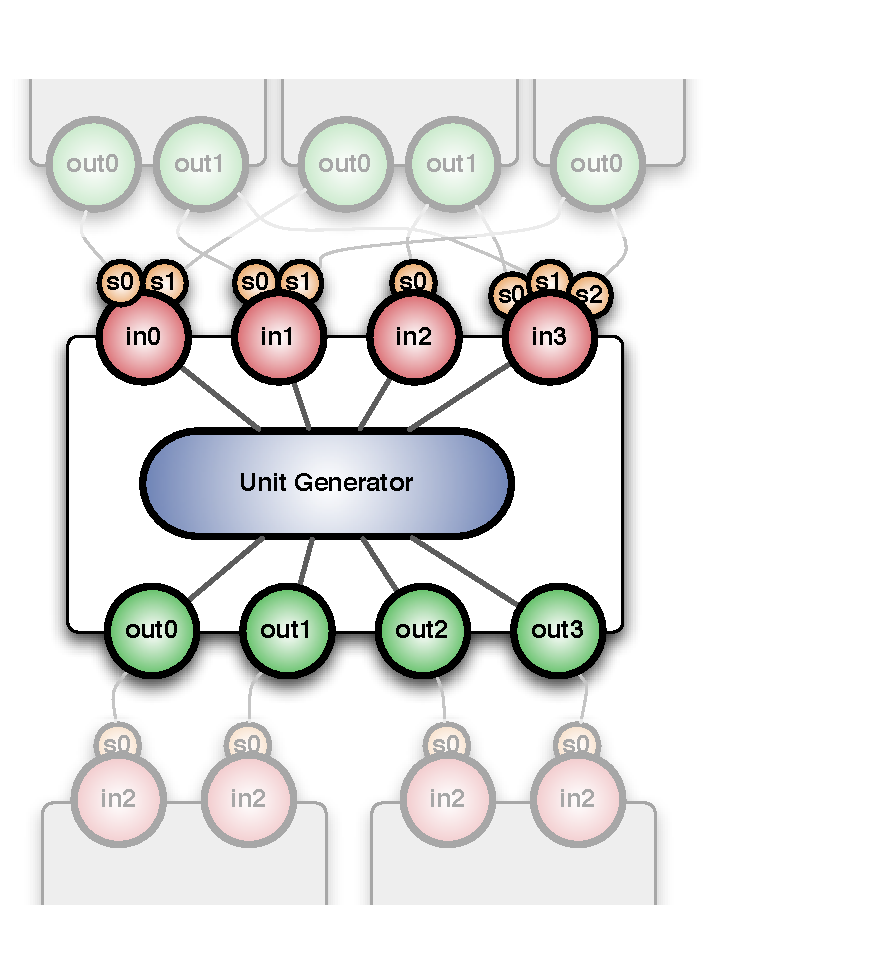
\includegraphics[width=0.9\columnwidth]{anatomy-compact}}}
\caption{TTAudioGraphObject Class Anatomy}
\label{fig:anatomy}
\end{figure}
%
\noindent The architecture of \texttt{TTAudioGraphObject} is layered: the audio graph object itself only knows about its inlets; the inlets only know about their sources (joins); the sources know from what object and from which outlet they are connected. 
In the figure this is illustrated by the object having four inlets. 
Two multi-channel sources $s0$ and $s1$ are connected to the first inlet $in0$, two to the second, and so on. 
In short:
\begin{tabbing}
\hspace{2.6cm}\=A graph has many objects.\\
	\>An object has many inlets.\\
	\>An inlet has many sources.\\
	\>A source has many channels.
\end{tabbing}
% From Rails book:
% Within the database, many-to-many associations are implemented using an intermediate join table. This contains foreign key pairs linking the two target tables. Active Record assumes that this join table’s name is the concatenation of the two target table names in alphabetical order. In our example, we joined the table categories to the table products, so Active Record will look for a join table named categories_products.

% (end)


\subsection{Building the Graph} % (fold)

For processing to occur, the connections of the graph must be established.  
This is accomplished by passing a reference to a source object, as well as the outlet and inlet numbers for the connection, to the downstream object's \texttt{connect()} method.  
Similarly, connections may be cut by passing the same information to the downstream object's \texttt{drop()} method.  
Connections may be created or dropped at any time before, after or during the graph being processed.  That is to day that there is no global signal chain compilation; the graph may dynamically change over the course of its operation and performance.

% TODO: Would it make sense to add that changes to the graph structure takes effect from the next frame processed? - TL

% (end)


\subsection{Processing the Graph} % (fold)

All processing is driven by the object at the end of the processing chain according to a two step process.  
First, a `preprocess' method is propagated up the chain from the terminal object.  
This zeroes buffers and sets flags that indicate each object's processing state.  
It is of no consequence if an object receives multiple preprocess calls, such as would happen if there are multiple terminal nodes.

Since Jamoma Audio Graph is using a pull-based architecture, an object's \emph{outlets} are passive.  
They are simply buffers storing the output calculated by the wrapped unit generator.  
The unit generator is simply an instance of a Jamoma DSP class, specified as an argument when the \texttt{TTAudioGraphObject} is instantiated. 
This unit generator is responsible for actually calculating the audio to be stored by the outlet buffers.

Unlike the outlets, the \emph{inlets} are active.  
When asked for a vector of audio by the unit generator, the inlets each request audio from each of their sources (other objects' outlets).  
If an inlet has multiple sources, those sources are summed.  
When all of the inlets have performed this operation, then the unit generator proceeds to process the audio buffered in the inlets and fills the buffers in the outlets.  
Sources manage a one-to-one connection between an inlet and an outlet; inlets may have zero or more sources.  
To summarize:

With the objects in the graph prepared by the \texttt{preprocess()} call, the audio can be pulled from the graph by a terminal object using the \texttt{process()} call on each of its sources.

% TODO: We need to discuss what we do in the case that one inlet have several sources with differing numbers of channels 

% Third, we could send a post-process message, but we don't at the moment.
% But what would the purpose of it be? What would this be able to do that could not just as easily be done as part of the next "preprocess" step? The only thing I can imagine currently that this would be useful for, would be to schedule asynchronous events. On second thought that might actually be useful, e.g. for updating GUI objects showing signal levels etc., or for banging control-rate events based on monitoring and analyis of audio signals... [TL]

% (end)


\subsection{Graph Description} % (fold)

Given an audio graph, the topology can be traversed for purposes other than directly calculating audio.  
Any node in an audio graph can be queried to create a description.  The returned \texttt{TTAudioGraphDescription} object will then provide metadata about the entire graph as seen through that object's inlets.  
There are many applications of this description, including visual representation of the graph, statistical analysis, and cross-coding.

% (end)

% (end)




%%%%%%%%%%%%%%%%%%%%%%%%%%%%%%%%%%%%%%%%%%%%%%%%%%%%%%%%%%%%%%%%%%%%%
%
\section{Application} % (fold)
%
%%%%%%%%%%%%%%%%%%%%%%%%%%%%%%%%%%%%%%%%%%%%%%%%%%%%%%%%%%%%%%%%%%%%%

% TODO: In section 1.1 Implementation we state that we have implemented JAG for Audio Unit. Don't Audio Unit then need to be added to this section? - TL

\subsection{Max/MSP} % (fold)

\begin{figure*}[!t]
\centering
\subfigure[Without Audio Graph, using MSP audio signals for 3 inputs and 16 loudspeakers] 
{\framebox{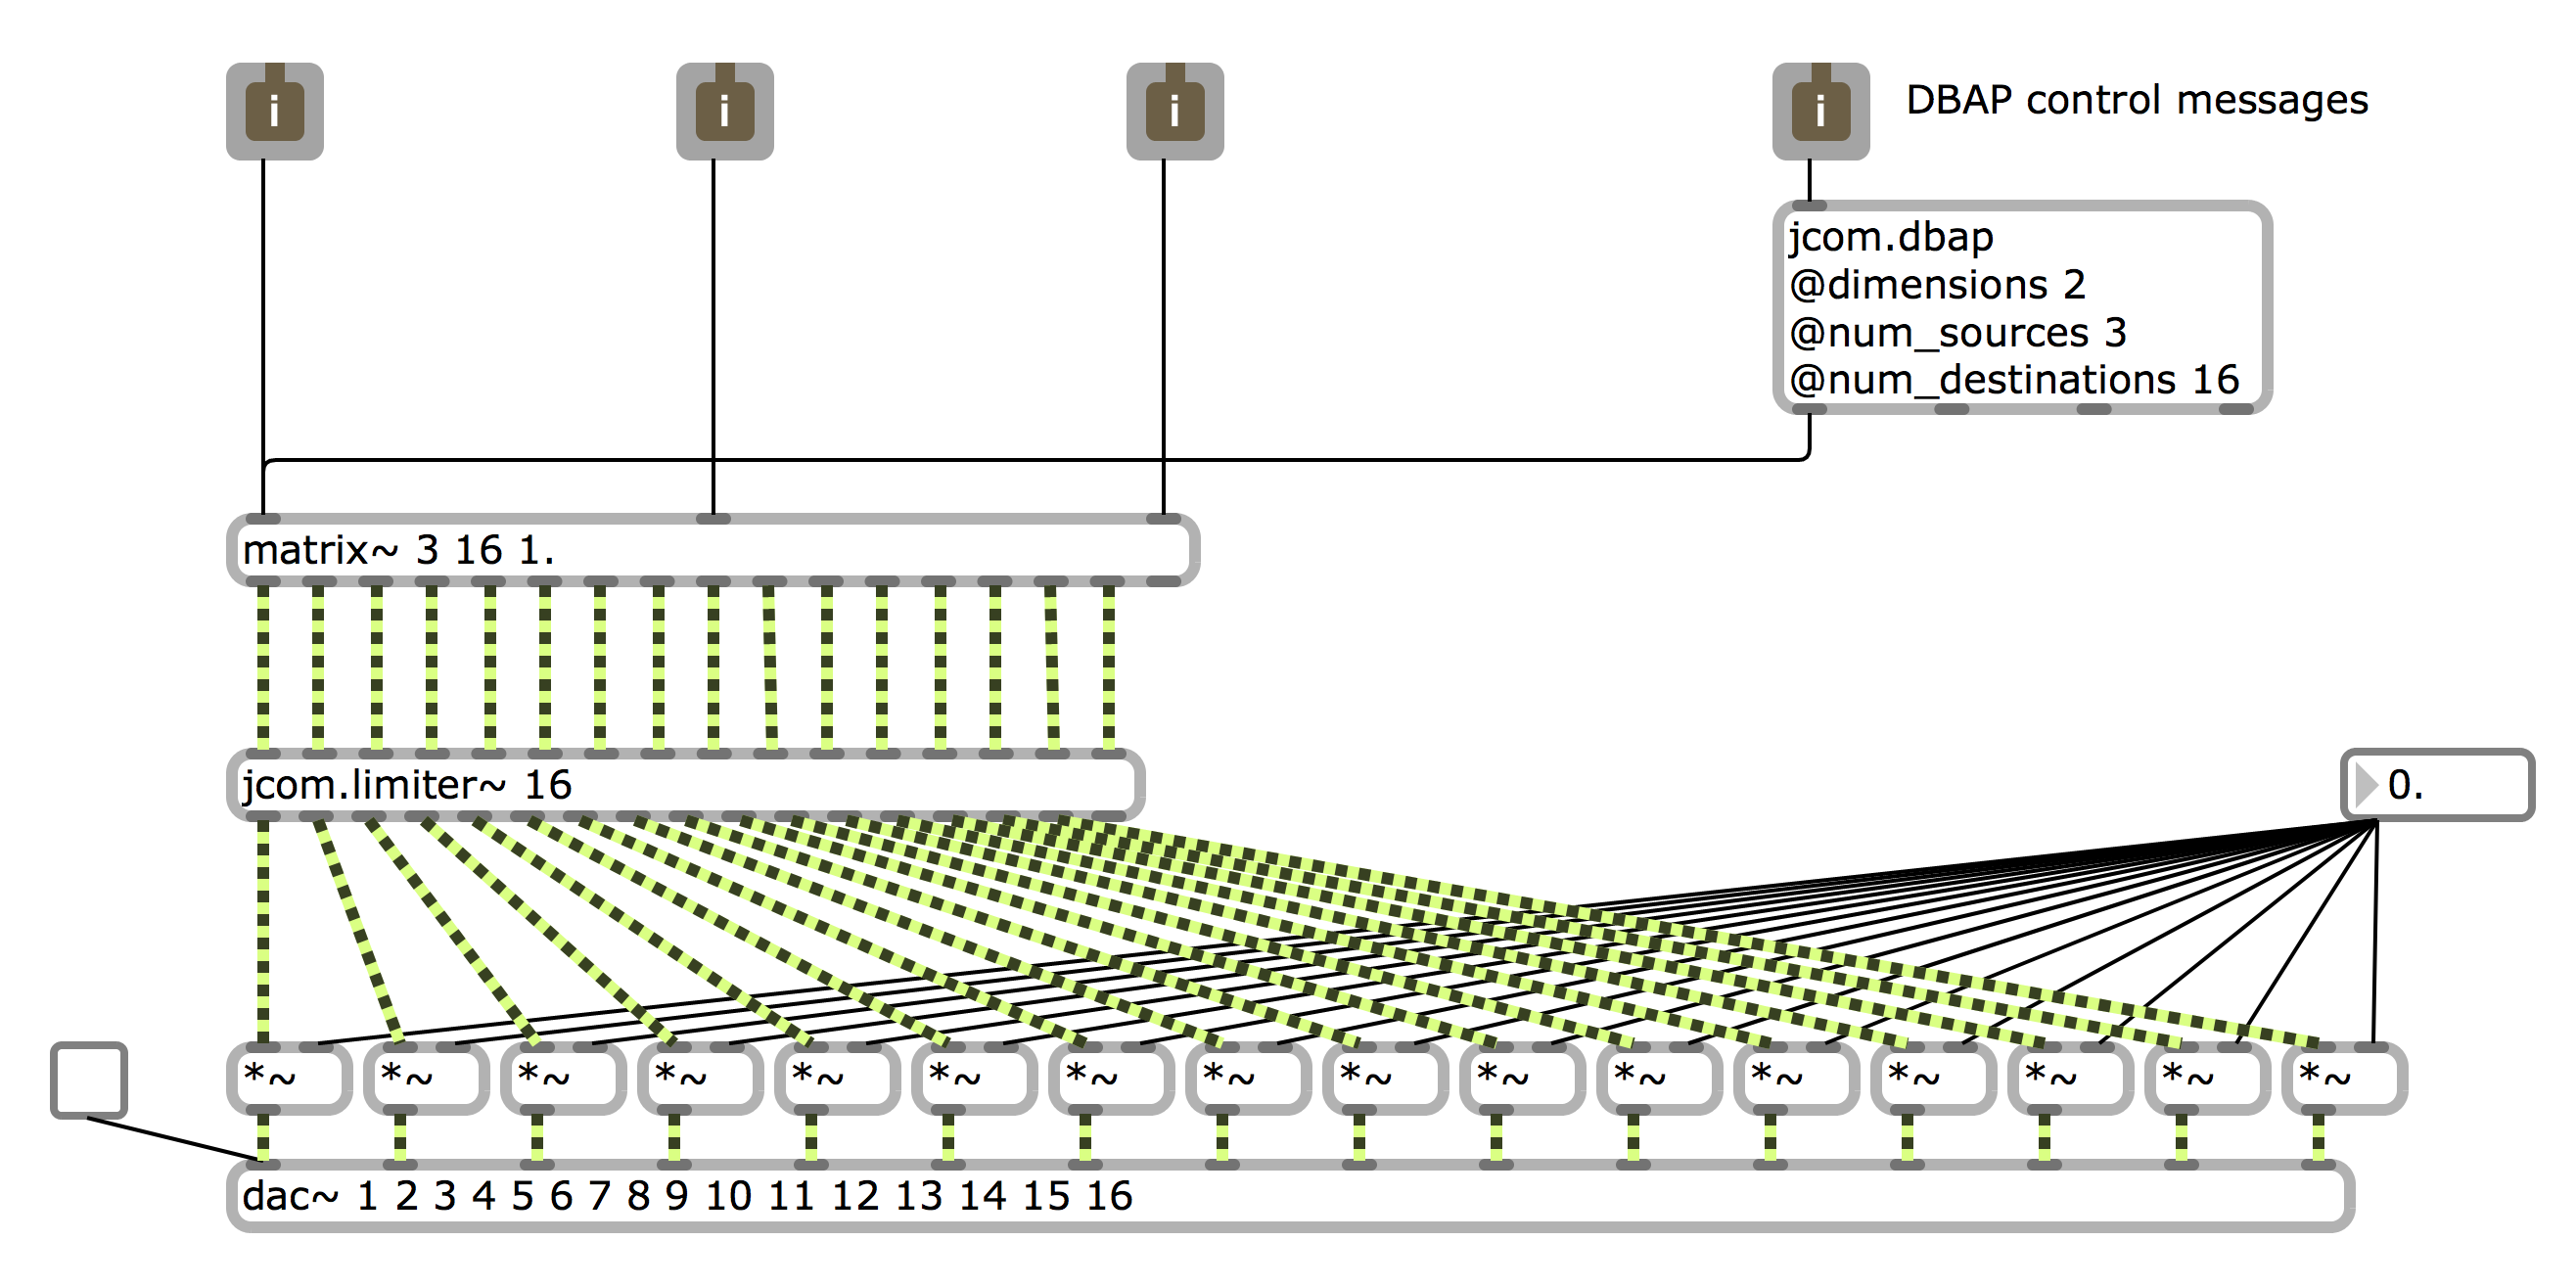
\includegraphics[height=0.225\textheight]{MaxBefore.png}}} \hspace{0.4cm}
\subfigure[With Audio Graph]
{\framebox{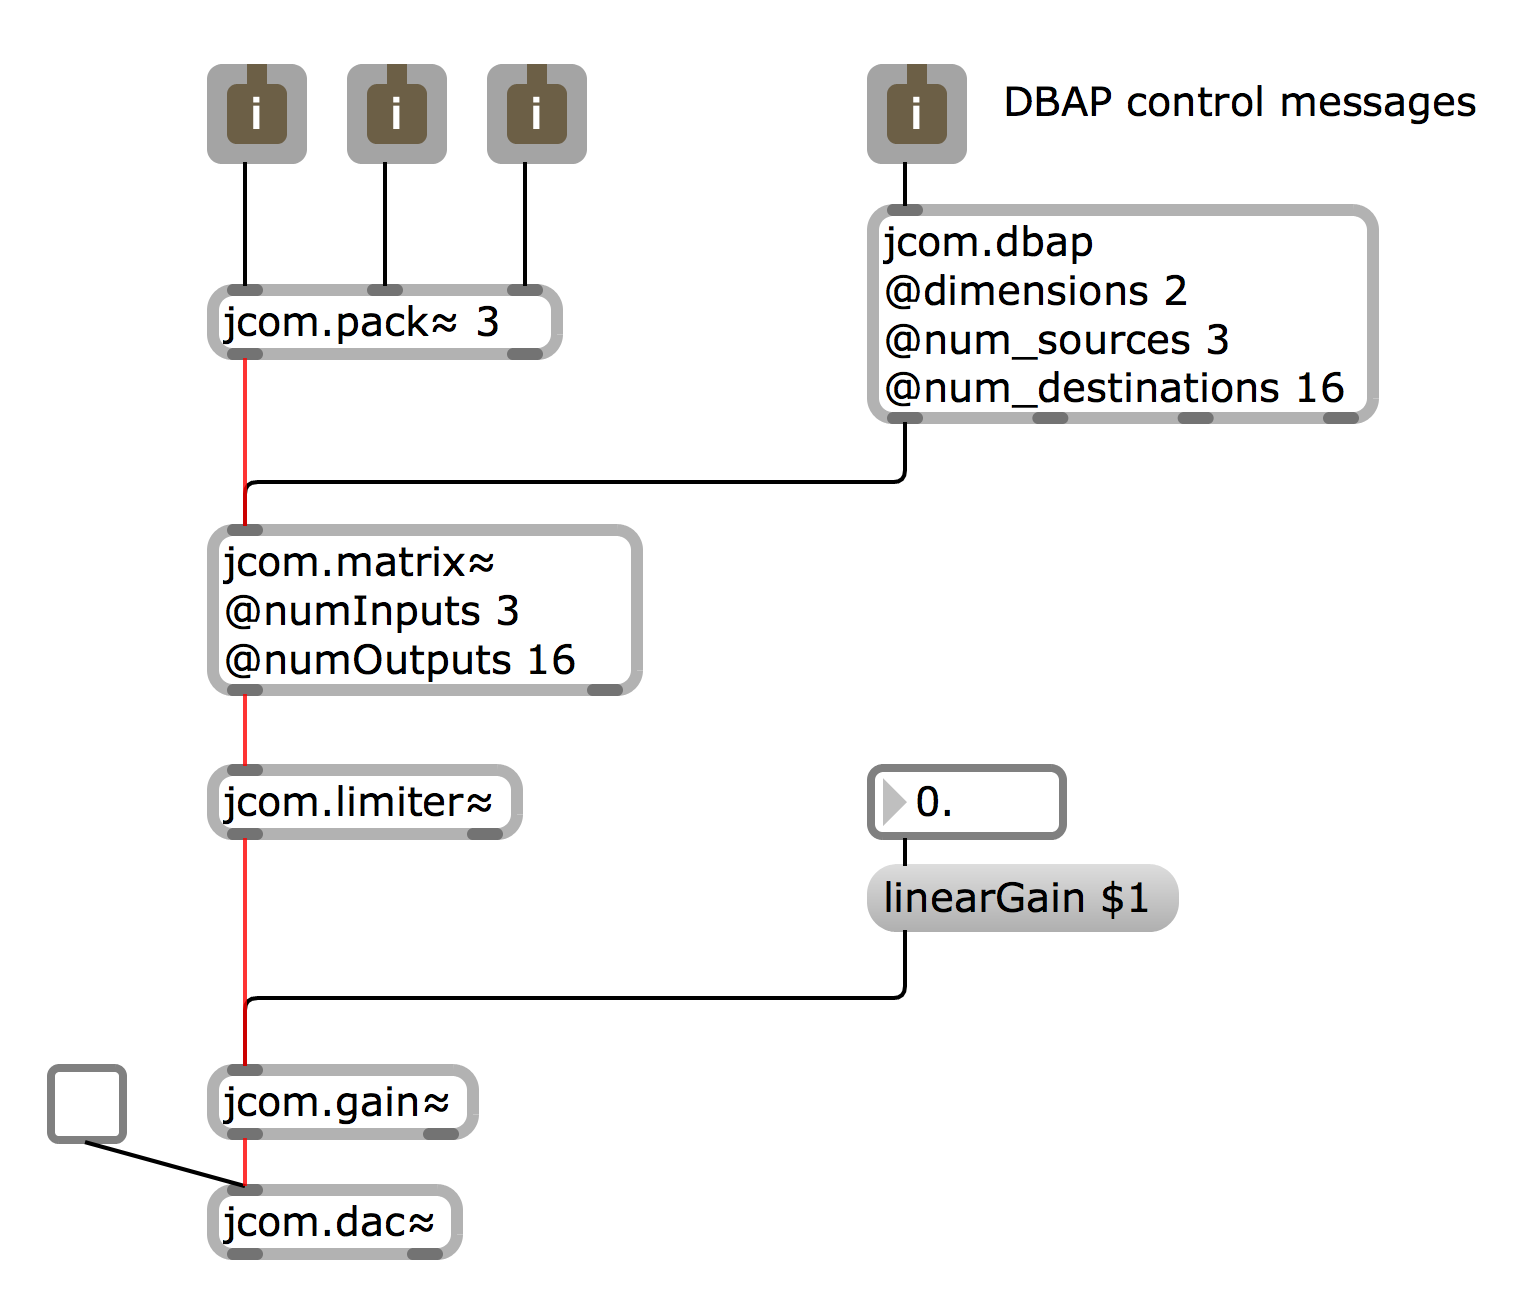
\includegraphics[height=0.225\textheight]{MaxAfter.png}}}
\caption{The Jamoma signal processing Max patch for Distance Based Amplitude Panning (DBAP)}
\label{fig:max-before-after}
\end{figure*}

A number of externals for multi-channel audio processing in Max have been developed combining Jamoma's Audio Graph and DSP frameworks. 
The Max implementation of the Jamoma Audio Graph represents multi-channel signals as ordinary patch chords.
Interfacing between MSP and a Jamoma Audio Graph is facilitated by the externals \emph{jcom.pack$\approx$} and \emph{jcom.unpack$\approx$}, packing and unpacking multiple mono MSP signals into and out of a multi-channel signal. 
\emph{jcom.adc$\approx$} and \emph{jcom.dac$\approx$} offers additional possibilities for direct audio input and output using PortAudio \cite{Bencina:2003}, bypassing MSP altogether. 
Two or more multi-channel signals might be intertwined into one joint multi-channel signal and separated again using \emph{jcom.join$\approx$} and \emph{jcom.split$\approx$}.
The sample rate and vector size used for Audio Graph processing as well as the number of channels in a multi-channel signal can be inspected using \emph{jcom.info$\approx$}.

A number of multi-channel audio generators and processors comprising common signal processing tasks are available. %for e.g. noise and common waveforms are available.
This set of generators can easily be extended.
The various units available in the Jamoma DSP filter and audio effects libraries can readily be wrapped into Audio Graph externals for Max.
\emph{jcom.fft$\approx$} and \emph{jcom.window$\approx$} were developed for spectral processing of multi-channel signals.
% TODO: Are further details required, e.g. on how to deal with complex signals (complex = complex numbers)?
% Currently a multi-channel signal is considered to be a complex signal with channel 1 being the real part and channel 2 being the imaginary part -- the design here has never really be discussed yet by us...  [TAP]
Several objects are available for level control and mixing: 
\emph{jcom.gain$\approx$} can be used to control gain levels for multi-channel signals, while \emph{jcom.matrix$\approx$} allows $M \times N$ matrix-based mixing of the $M$ channels of the incoming signal onto the $N$ channels of the resulting signal. 
This can e.g. be used for various amplitude-based spatialization algorithms such as VBAP \cite{Pulkki:1997vbap}, DBAP \cite{lossius:2009} and ambisonics \cite{Schacher:2006ambi_max}.
Finally \emph{jcom.matrixmixer$\approx$} offers possibility of mixing $M$ incoming multi-channel signals onto $N$ returned multi-channel signal.
This combined mixer/router is still rudimentary, and assumes all incoming and returned signal to have the same number of channels.

Figure \ref{fig:max-before-after} illustrates the use of Jamoma Audio Graph objects in a patch providing spatialization of 3 mono sources to 16 speakers, with additional post-spatialization mastering of the signals using a limiter and gain adjustment.
The use of JAG objects greatly helps simplifying the patch as compared to a standard MSP audio graph. 

% TODO: Finish of this section by referencing \ref{fig:max-before-after}, how it illustrates MSP to Audio Graph bridging, matrix, FX and output using PortAudio. Also comment on how much simpler it is to reconfigure the number of speakers: We now only need to change attribute values in jcom.matrix≈ and jcom.dbap, instead of having to do repatching. (Save latter for discussion)

%\begin{figure*}[!t]
%\centering
%\subfigure[Without Audio Graph, using MSP audio signals for 16 inputs and 12 loudspeakers] 
%{\framebox{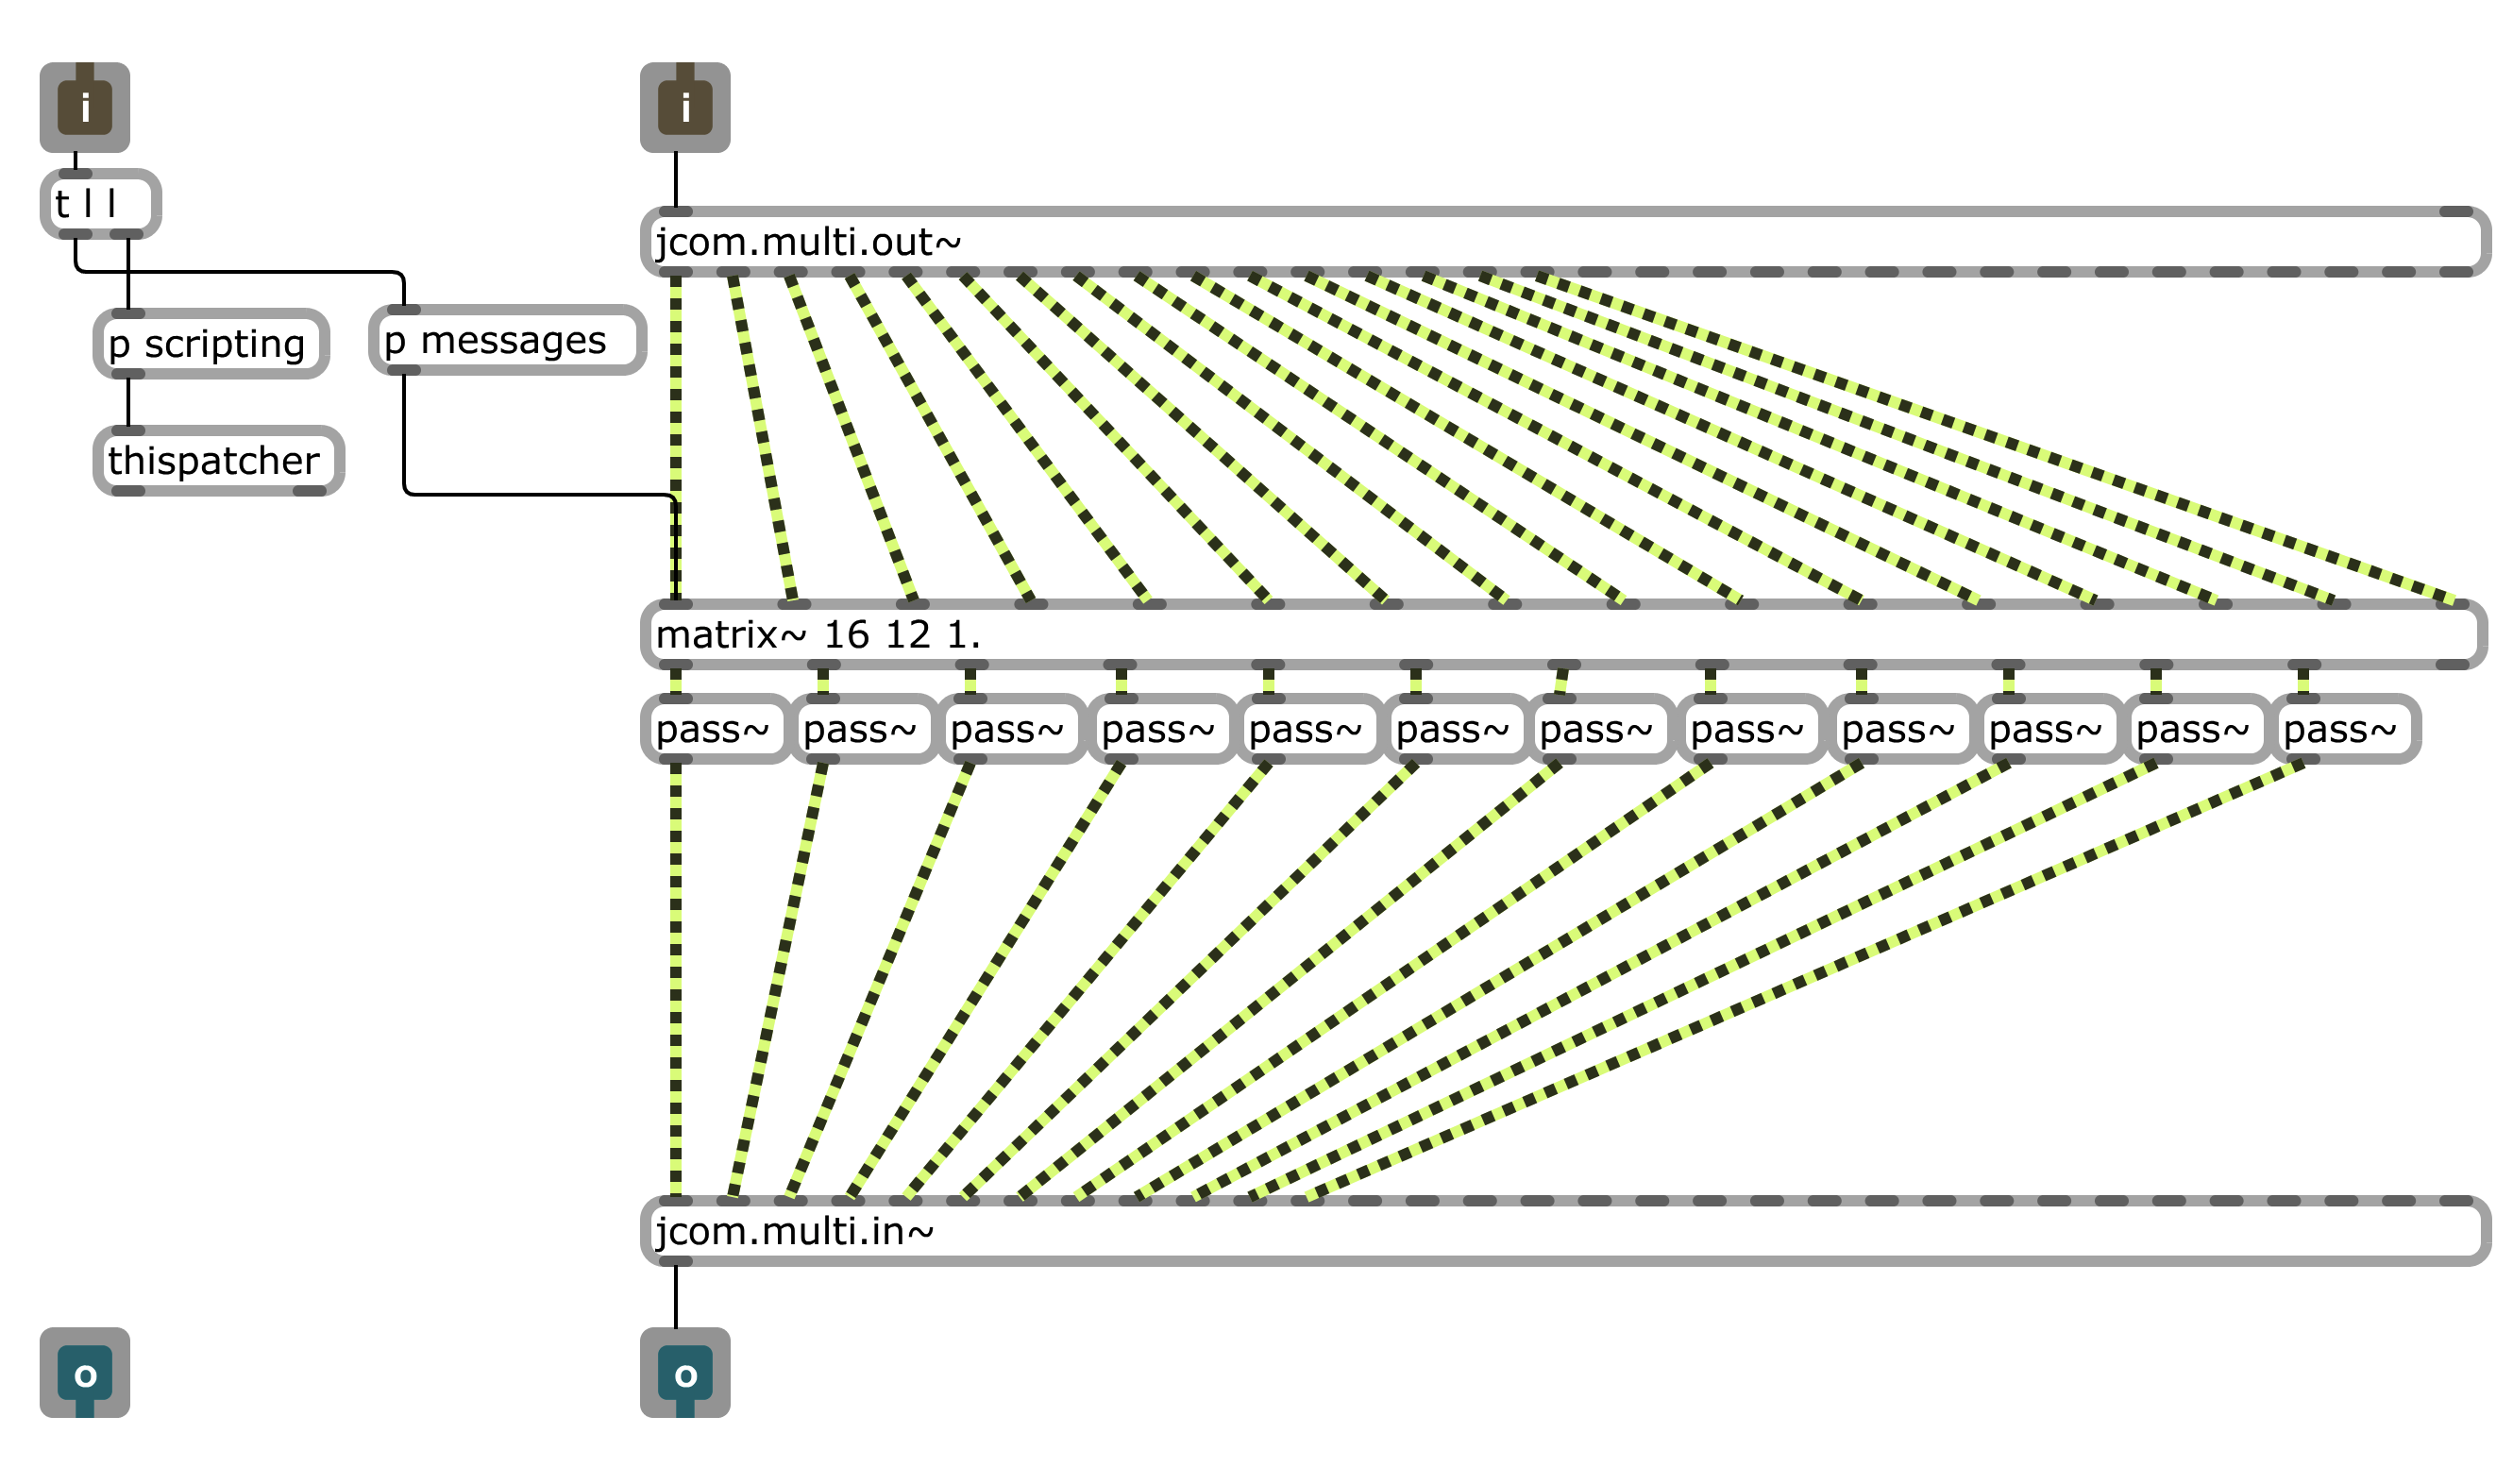
\includegraphics[height=0.28\textheight]{jalg-sur-vbap-before.png}}} \hspace{0.7cm}
%\subfigure[With Audio Graph]
%{\framebox{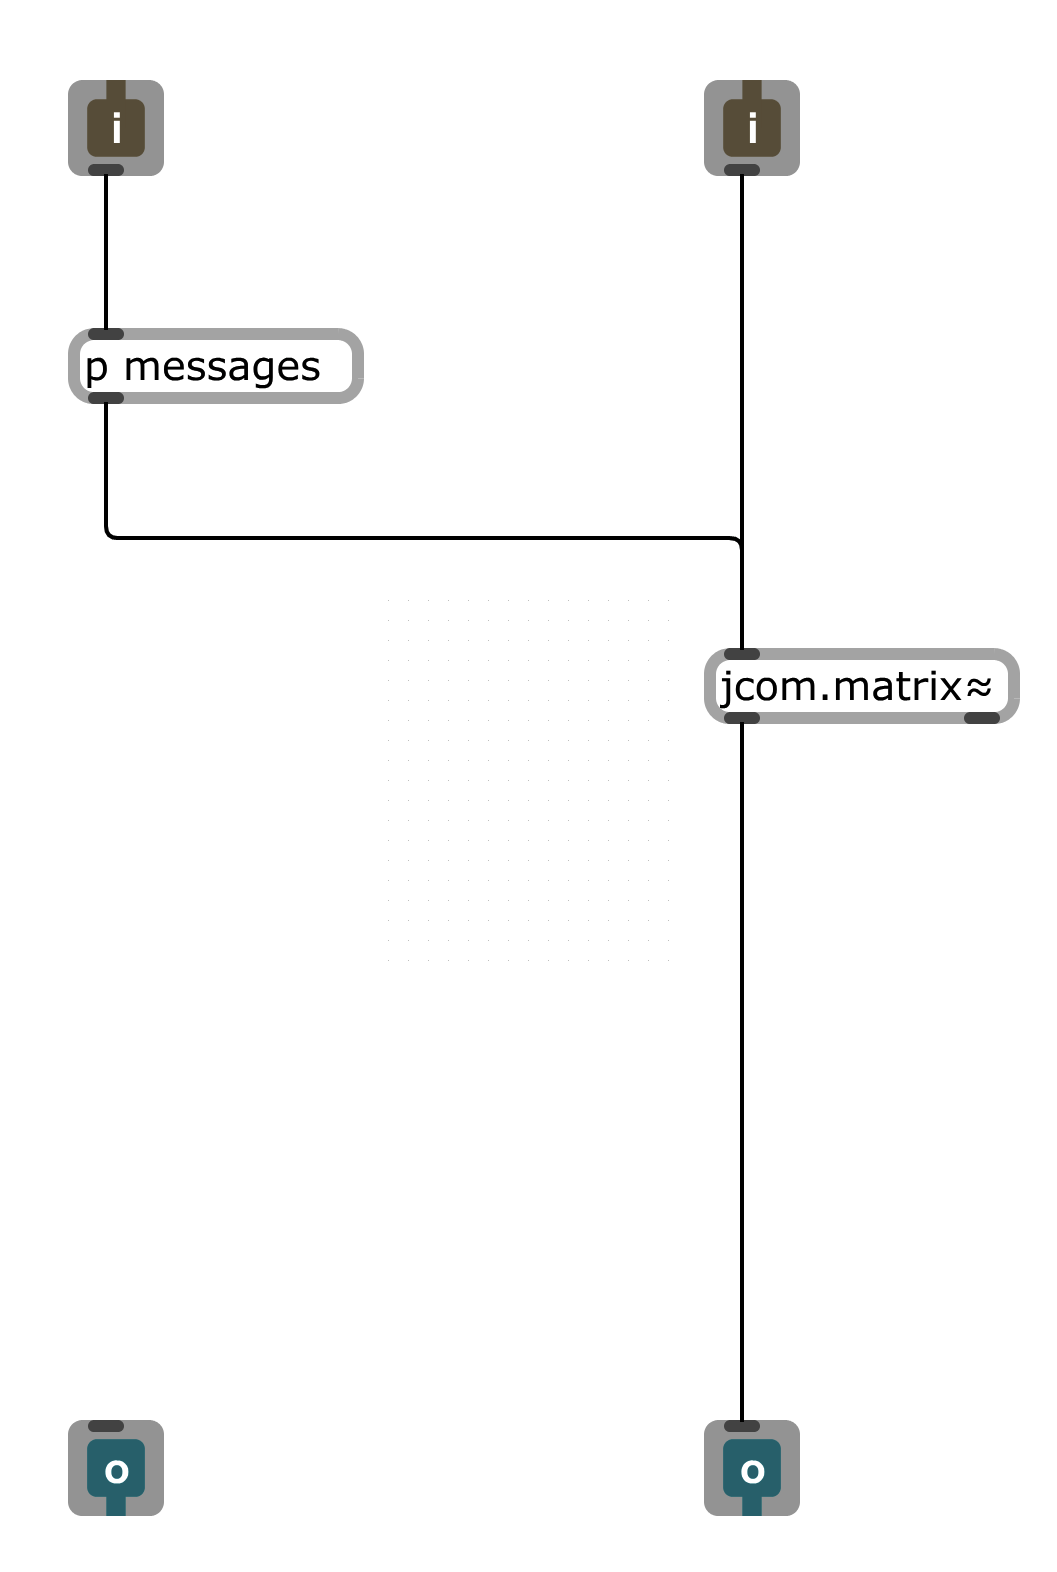
\includegraphics[height=0.28\textheight]{jalg-sur-vbap-after.png}}}
%\caption{The Jamoma signal processing Max patch for Vector Base Amplitude Panning (VBAP)}
%\label{fig:max-before-after}
%\end{figure*}

\subsubsection{Jamoma Modular} % (fold)

%TODO: I find the way we move between present and past tense in the following paragraph awkward. - TL
A strong component of the Jamoma Modular framework is the provision of ready-to-use building blocks for sound spatialization \cite{Peters:2009}.
To pass multi-channel signals between these modules, Jamoma up until now has been using a simple patching hack that wraps multiple MSP signals into a multi-channel cable. Within each module, this multi-channel connection was then unwrapped in order that audio signals could be processed. 
One of several disadvantages of this solution was that whenever the number of sources or speakers was changed, MSP objects and connections had to be destroyed and created.
As Jamoma modules for spatialization aims at being flexible, enabling the user to define the number of incoming (to be spatialized) sounds and number of outgoing audio feeds (number of loudspeakers), creating and deletion of MSP objects and connections was done using scripting.
This could create certain stress on Max for time critical situations, and was not experienced to be sufficiently reliable for real-world performance situations.
Furthermore a change in the DSP structure also required a rebuild of the DSP chain.

The previous scripting and patching hack approach is currently being replaced by Jamoma Audio Graph externals to simplify the spatialization modules and make them more robust.
Figure \ref{fig:max-before-after}b indicates how the number of sources and speakers can be changed simply by updating attribute values for a few select JAG externals, thus eliminating the need for scripting in Jamoma Modules.
Because the Audio Graph signal network can be dynamically reconfigured without the need to recompile the DSP signal chain, on-the-fly changes are possible while audio is running.

% CHANGED: I think we most of the following more or less covered now, but it should be breviews. I see some that fit better in a future work section.

% Some important things to keep in mind:
% - Priorities, how to we control the order of operations?    We don't at the moment (which is like Pd, but unlike Max)
% - Matrix mixer/router development, with particular thought about what happens when 5.1 audio is routed to stereo etc.
% - Signals of varying data rate (for example as proposed by Pulkki), e.g. compressed signals or higher res signals
% - Signals of steady data rate but varying vector/buffer size (as in FTM/Gabor)
% Dynamic number of channels (perhaps useful for FFT and spectral processing?)
% Would be ideal if we could have a wrapper for standard MSP external objects as Audio Graph objects. 
% Call the DSP method directly from this wrapper?
% Create our own internal DSP chain for it?
% start simple as with biquad~, meaning 1 in and 1 out...
% it seems like the easiest way out is to just use patcher scripting.

% One difference to Max/MSP and Pd is that the signal network can be reconfigured dynamically without requiring a 'recompile' of the signal chain.  
% This is addressed through Jamoma Audio Graph -- Jamoma DSP is low level and is agnostic about how objects are combined into a network or topology.

% (end)
% (end)

\subsection{PureData (Pd)} % (fold)

The Jamoma Audio Graph layer is also implemented for Pure Data, which is essentially similar to Jamoma Audio Graph for Max/MSP. 
The most obvious difference between JAG for Pure Data and JAG for Max may be the slightly different naming convention, the Pure Data version using `=' instead of `$\approx$' appended as an indicator for multi-channel signal streams. 
Figure \ref{fig:pd} demonstrates the use of Jamoma Audio Graph in Pd for passing 4 channels through a chain for processing, taking advantage of the multi-channel patch cord connections.  

\begin{figure}[htbp]
\centerline{\framebox{
	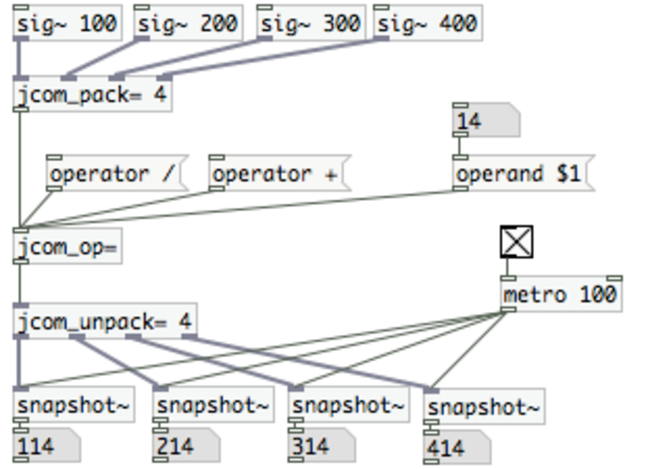
\includegraphics[width=0.7\columnwidth]{multicore-pd}}}
\caption{Pd patch, processing 4 channels with Jamoma Audio Graph}
\label{fig:pd}
\end{figure}

% (end)


\subsection{Ruby} % (fold)

Jamoma Audio Graph is ideally suited for use in many different environments. 
This includes not only graphical environments, but textual environments as well.  
The authors have created an implementation of Jamoma Audio Graph for the Ruby language environment.  
Ruby offers a wealth of application areas include web development using Ruby On Rails \cite{Ruby:2009} and Live Coding \cite{Collins:2003} using \emph{irb}.  
The following listing demonstrates a simple \emph{irb} session:

\begin{lstlisting}
  require 'TTRuby'
  dac = TTAudio.new "multicore.output"
  osc = TTAudio.new "wavetable"
  dac.connect_audio osc
  dac.send "start"
  osc.set "frequency", 220.0
\end{lstlisting}

\noindent By using Jamoma Audio Graph in the Ruby environment for live coding, users are able to access all of the benefits of using a popular, general purpose language while at the same time gaining access to many of the benefits of a domain specific language for musical performance such as ChucK.

% TODO: Are there any published articles specifically about using irb for live coding performance?
% TODO: Trond, there is a chapter in this book: http://books.google.com/books?id=93y-8DRUAz8C&lpg=PP1&ots=5_8bnjZqxB&dq=live%20coding%20irb%20ruby&lr=&pg=PR10#v=onepage&q=live%20coding%20irb%20ruby&f=false
% What do you think?

All features of Jamoma Audio Graph can be accessed in real time through a web browser using Ruby on Rails.  Through the use of AJAX, interactive widgets can populate a dynamic interface in a web-browser for real time control of parameters, as in the screenshot below.

\begin{figure}[htbp]
\centerline{\framebox{
	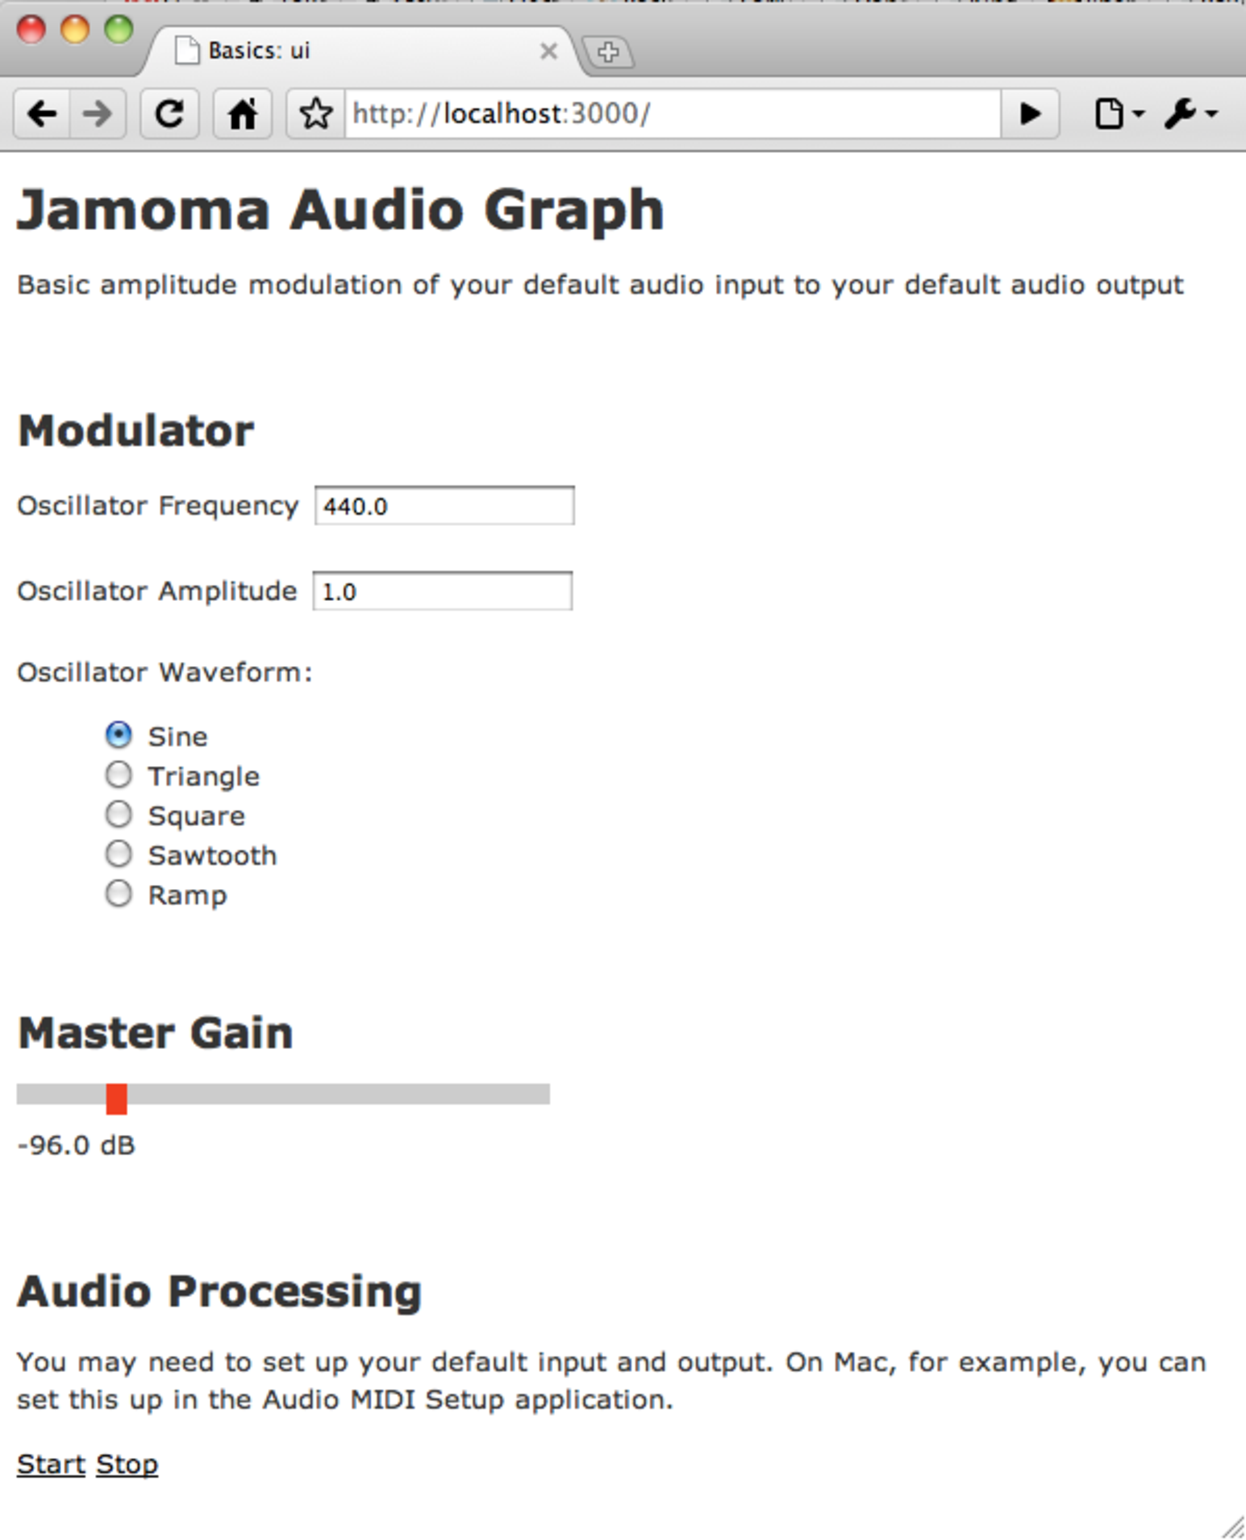
\includegraphics[width=0.7\columnwidth]{multicore-rails}}}
\caption{Jamoma Audio Graph graph operating in a Ruby on Rails application through a web browser}
\label{fig:rails}
\end{figure}

% (end)


\subsection{Cross-Coding} %(fold)

Using the capabilities of a graph to produce a description of itself, we are able to port code across environments in a variety of formats.  
For example, we have implemented functions that export a graph created in Max to a Ruby source file.  
Likewise we can export from a Ruby source file to Pd and from a Pd canvas to C++ code.  

The ability to export code/patcher/canvas/document from any supported environment to any other supported environment offers great flexibility, not only for code generation and prototyping, but for freedom in sharing work across platforms and with colleagues.  
The currently supported export formats are: Max 5 patcher, C++ source code, Ruby source code and Pure Data.

The additional ability to compile code and export a ready-to-use AudioUnit or VST plug-ins from any of these environments is currently in active development.

% (end)
% (end)




%%%%%%%%%%%%%%%%%%%%%%%%%%%%%%%%%%%%%%%%%%%%%%%%%%%%%%%%%%%%%%%%%%%%%
%
\section{Discussion and future work} % (fold)
%
%%%%%%%%%%%%%%%%%%%%%%%%%%%%%%%%%%%%%%%%%%%%%%%%%%%%%%%%%%%%%%%%%%%%%

\subsection{In Practice} % (fold) Practical Considerations
% how is it to work with

Audio processing is demanding on several levels.  
Computational efficiency and performance concerns are just a few of the aspects related to the real-world use and development of any audio graph framework. 
The Jamoma Audio Graph framework seeks to strike a balance between raw number-crunching, coding and maintaining code, as well as the flexibility and usability of features for end-users in various environments.


\subsubsection{Code design} % (fold)

The Jamoma frameworks align with contemporary philosophies for good coding practice, thus facilitating the readability, debugging, maintenance and distribution of code.
The frameworks emphasize expressive syntax, idioms, and conventions \cite{Martin:2009} and adhere to the DRY (Don't Repeat Yourself) principle, which states that ``Every piece of knowledge must have a single, unambiguous, authoritative representation within a system'' \cite{Hunt:1999}.
Unit testing  \cite{Martin:2009} is so far implemented only in some of the frameworks, mainly for methods processed asynchronously, at control rate.
A general system for developing methods for testing audio signal processes and graphs remains to be developed, but is likely to be much simpler to achieve using the text-based Jamoma Audio Graph implementation for Ruby than it would be within the graphical patching environments Max or Pd.

The emphasis in code design is a long term investment in making the frameworks pleasant to work with and on, keeping the code base intuitive to use, maintainable, well-documented, stable and extendable, thus hopefully also encouraging others to make use of the frameworks and join in contributing to future development.

% +1 : nice job on the above, Trond!  :-)    [TAP]

% TODO: not sure how boastful we really want to be with the above -- testing and documentation are currently anemic (at best).  [TAP]   (but, this is future work)  -- what does it really mean that this is pleasant to work with

% Eric Lyon had the following comment about our DSP paper, which I think could be worked-in here as a way to tie the goals of Audio Graph into the bigger picture:
%
%	I'm most intrigued by this statement, and would be happy to hear more about it in your paper:
%
%		"Perhaps more important, but more difficult to quantify,
%		we believe we have created a context in which code is ``pleas-
%		ant to work with.''
%
%		This seems to be an increasingly important criterion, especially if (as I believe) we're evolving to a much more porous and flexible continuum across data-flow, scripting, and compiled coding as different entry points for musicians, depending on what they need to do. 

% (end)

\subsubsection{Audio graph patching} % (fold)

% Assigned to Trond

The initial motivation for development of Jamoma Audio Graph was simplification of work on spatialisation in Jamoma Modular. 
The use of multi-channel signals greatly reduce tedious and repetitious patching where the same chain of audio processes have to be created over and over again for each channel. 
More important though it greatly improves the workflow in terms of flexibility and inter-operability.
Jamoma modules for spatialisation shares a common interface, and the number of sources and speakers can be dynamically reconfigured on the fly in a simple way using configuration scripts describing the number and positions of sources and speakers. 
The usefulnes of this can be illustrated by the practical experience of one of the authors while working on a sound installation in Oslo in 2002 \cite{Rudi:2003}.
For the last week before the opening, two of the composers moved several times a day between working at the installation site using a 24 speaker setup, a 16 speaker setup at the studio of one of the composers and using stereo headphones.
Every time the parts of the patch dealing with spatialisation had to be substituted.
Using Jamoma Modular it would instead be possible to trigger simple cue scripts to reconfigure the system from one setup to another.

Within Jamoma Modular the Jamoma Audio Graph is eventually planned to be used for all audio modules.
One of the major benefits will be the ability to easily reconfigure each module for work on mono, stereo, 5.1 or other surround sound signals.
This way we avoid having to create and maintain several versions of modules for the same audio process, in accordance with the DRY principle.
For modules that also depend on the use of ordinary MSP externals internally, we still will have to use \emph{jcom.pack$\approx$} and \emph{jcom.pack$\approx$} in combination with Max scripting.




- ability to export to other environments (C++, Pd, Ruby, AudioUnit plug-ins)
- Integra is striving somehow for a similar cross-coding....

% (end)


\subsection{Performance} %(fold)
% TODO: How to avoid the musical performance connotation in title?
% Maybe subsubsections break this apart?

CPU concerns:

- not very optimized right now, due to the early state of the project

%- Integrated Analysis and Benchmarking -- perhaps reference the upchuck operator in ChucK?
 %  -- This integrated analysis and benchmarking could also provide the basis by which an audio graph such as Jamoma Audio Graph is able to evaluate how to optimize the processes in the graph to make intelligent decisions on how to distribute the processing among threads or processors.
 
Other performance concerns:

- performance is a question of CPU use, but also how it performs in other senses....
- dynamic patching without breaking audio
- benefit of live coding paradigm:
    - performance patch: be able to create and delete subpatches on the fly depending on what's required for different parts of the performance
    - alternative way of freeing up CPU to the mute~ or poly~ approach in MSP
    - will it be easier to make polyphonic synths (one obejct can make several instances internally, and then get them all onto the same multicable)
    - polyphonic synthesis: voices are represented as dynamically changing channels in a portion of the graph, which are mixed at the end using a matrix=. Sort of similar to what Csound do: Creatind and destroying instrument instances as needed rather than having a fixed number of voices (the way poly~ have)

%
%		A few other thoughts - maybe worth writing a bit more on SuperCollider, as it is much more flexible and elegant than Max/MSP/Pd in allowing new pieces of DSP to be eased in and out of a performance (compared to the rigid poly~ structure, on the one hand, or glitches whenever new DSP objects are created on the other). 

% (end)

\subsubsection{Multithreading} % (fold)

Parallel CPU architectures are becoming increasingly common in desktop computing platforms.
UC Berkeley's Parallel Computing Laboratory identified audio applications as one of the most promising but also most challenging use cases for parallel computing \cite{asanovic2008parallel}. 
In addition to prevention of race conditions and deadlocks, multi-channel real-time audio computing also requires low latency and jitter-free audio processing execution.

Jamoma Audio Graph supports operation in multi-threaded environments by running multiple parallel graphs on separate threads.  Current research is focused on the expansion of multi-threaded support to include intelligent and adaptive multi-threading within a single graph structure.  

The implemented pulling strategy (Section \ref{sec:pull}) offers opportunities to analyze and benchmark at the audio graph structure in real-time.  Involved audio processes can then be distributed and managed amongst different threads or processors, particularly where bifurcations of the graph are present, based on a heuristic determination of how to best balance resources against computational load.  A promising management strategy can be found in \cite{PartzschAES122}.

% TODO: Nils, I assume the above citation is from you?  Can I get a copy of this so that I know what you are talking about?  Thanks!  [TAP]

%The structure of Jamoma Audio Graph is ideal for distributing processing of the graph amongst parallel threads.  
%More powerful and dynamic opportunities arise when a graph itself is distributed to parallel threads.  

% CHANGED: I think the next sentence is more than obvious [TAP]
% Besides real-time processing, also the execution speed in off-line rendering can benefit from parallel processing. Future work includes testing Jamoma Audio Graph in non-real-time situations.

%wouldn't Audio Graph (on its own) greatly simplify non-realtime processing, provided that we had audio objects for anything needed so that we could totally avoid MSP, and also had a way of controlling the Max clock?

%    - multi-threading where applicable
%    - pragmatic multi-threading: real-time statistics for optimizing between different processors
%   
%A   B
% \ /
%  C

% TANGA provides and interesting environment because the audio engine is explicitly multi-threaded and thus multi-core capable\cite{Reiter:2007}.  However, it doesn't fit the bill because it is targeted at one context: MPEG-4 scene rendering.  We need something more general.  And it doesn't matter because we are thread-agnostic.

% (end)
% (end)

\subsection{Flexible audio graph management} % (fold)

\subsubsection{Multiple Simultaneous Graphs} % (fold)

By it's nature, an audio graph is defined as all objects connected together into a graph structure terminating at a terminal object that drives the graph.  
There is no limitation on how many of these graphs may exist independently, and simultaneously, in any environment.  
As these graphs are fully-independent of each other they may run at different rates, in different threads, and addressing different hardware.  The independent graphs may even run side-by-side with one running in real-time while another is operating out of real time.

% (end)


\subsubsection{Dynamic vector size} % (fold)

% TODO: assigned -- Trond

One example the demonstrates the need for dynamic vectorsizes is the gabor.psola.pat example from FTM. 
Also granular approaches may benefit (for example, implementing some of the ideas from Curtis Roads' engine).

- ideal environment for spectral processing (changing signals into the native FFT size)
- similar for granulation.... (creating/destroying grains on-the-fly, dynamic vector sizes)
- Trond making things difficult: Would we somehow need to ID-tag each channel, so that a filter downstream from a saw generator recognize which channel it is dealing with

% TODO: I have no idea what Trond is talking about in the above :-)  [TAP]

% (end)


\subsubsection{Implicit Patching} % (fold)

Currently all connections in an audio graph are managed manually.  In a graphical environment such as Max we could re-phrase this to say that the connections between objects are explicitly patched together by the user.  A higher-level alternative to this ``explicit patching'' by the user is the ``implicit patching'' paradigm embraced by Marsyas \cite{Bray:2005}.

With implicit patching the user is able to interact with groups of objects that are networked together by specifying a pattern to use, rather than directly and manually making each connection.  
One elementary example is the creation of a multi-band EQ, by creating an array of bandpass filters and then specifying then to connect as a parallel group.  
A group patched according to a `series' pattern would connect one after the other to apply a transformation throughout the chain of objects in the group.

% (end)

% (end)


\subsection{Improving support for work on spatial audio} % (fold)
% TODO - assigned to Nils
The advantages in working and maintaining of multi-channel audio patches in common computer music environments can be clearly seen in Figure \ref{fig:max-before-after}. 
For now, the ability to work individually on a single audio channels within the audio graph is limited.
For instance, it is possible to apply jcom.filter$\approx$ to manipulate all audio channels within a graph connection in the same way. However, many multi-channel audio application (such as the Near Field Compensation in Higher Order Ambisonics) rely on filtering processes individualized across audio channels. Future work will address this issue.

We also want to include upmix/downmix algorithms into the Audio Graph to seamlessly mediate between different kind of multi-channel media formats including compressed spatial audio material (e.g. mp3-surround, DIRAC). Here, we are planning to explore the potential to attach additional meta-information to the individual audio channels to ensure that the correct audio material is being processed (e.g. to identify the signals in an Ambisonics B-format, or to distinguish a binaurally processed audio stream from a conventional stereo track). 

Somehow related to IEM's CUBEmixer \footnote{\url{http://ambisonics.iem.at/xchange/products/cubemixer}}, the authors are currently developing a multi-channel authoring/mixing application which enables the user to work and combine common spatial audio rendering concepts such as VBAP, DBAP, ViMiC \cite{Peters:2008b} and Ambisonics according to his compositional aspiration and/or technical possibilities \cite{Peters:2009}. The Jamoma Audio Graph Layer is essential to this development and is already being used in a prototype of this application (Figure \ref{fig:SceneMixer}).
\begin{figure}[htbp]
	\centering
		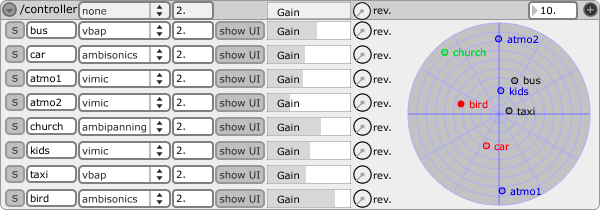
\includegraphics[width=1\columnwidth]{SceneMixer.png}
	\caption{Prototype of an authoring application combining common spatial rendering concepts using Jamoma Audio Graph}
	\label{fig:SceneMixer}
\end{figure}

% == Mighty Mixer ==
% stuff to work on:\\
%- how do we dynamically change the number of channels on the fly within one mulichannel signal? use a jcom.matrix=, jcom.split=, add a jcom.duplicate= ? 
%- can multicore cabels contain additional meta-information (attributes, dictionaries....)
%- encoded audio? (AAC, mp3-surround, DIRAC) , or ... does multicore only works with PCM audio ? -- we need to be %able to specify stream-format metadata (also for 7.1 vs 8-channel)
%- how we do upmixing/downmixing of channels ? 
%    - spatialization - currently prototyped:
%        - VBAP: matrix= so no scripting, 
%            numSource -> numInputs
%            numSpeakers -> numOutputs
%        - todo: ramping
%        - future: making spatialisation objects will contain an instance of the matrix= object
%        - this way we have access to spatialisation in all environments
%            (and some of them are available only in some of the environments)
%        - even more into future: matrixmixer (mighty mixer): creates one instance for each inlet to outlet coupling
%                                    
%        - also into future: same for ViMiC combining matrix=, delays, etc.
%        - we have a prototype implementation in Nils' object (userLib->Vimic->jmod.sur.sourceControl.maxhelp)

% (end)
% (end)




%%%%%%%%%%%%%%%%%%%%%%%%%%%%%%%%%%%%%%%%%%%%%%%%%%%%%%%%%%%%%%%%%%%%%
%
\section{Conclusions} % (fold)
%
%%%%%%%%%%%%%%%%%%%%%%%%%%%%%%%%%%%%%%%%%%%%%%%%%%%%%%%%%%%%%%%%%%%%%

We rock.

% (end)




% CHANGED Trond's attempt at outlining ends here  -------------------------------------


%%%%%%%%%%%%%%%%%%%%%%%%%%%%%%%%%%%%%%%%%%%%%%%%%%%%%%%%%%%%%%
%
% The below seems to be leftovers and snippets from the section reviewing other solutions, as well as odds and sods:
%
%%%%%%%%%%%%%%%%%%%%%%%%%%%%%%%%%%%%%%%%%%%%%%%%%%%%%%%%%%%%%%

% TODO: we need an object like out≈ that drives a graph outside of real time to fill a buffer~ or jit.matrix
% TODO: trond or nils -- do you have some interesting applications of the above?
% TODO: If we are presenting a graph system, should we discuss the potential (if any) for expanding this from being a graph system for audio processing, to video processing or other kinds of time-tagged data, along the line of e.g. Max/Jitter, QuartzComposer or Octane?
% TODO: Discuss the potential for work on spatialisation, and further work in this direction...
% TODO: Non-PCM streams?  The need for audio signal metadata?
% TODO: Also talk about the Jamoma Graph thing?

% TODO: Grand Central Dispatch (GCD) is now open source, is this relevant?

% unit generators are added to a collection and their interaction with the signal processing graph is determined according to a pattern such as 'series', 'fanout', etc. \cite{Bray:2005}.

%Marsyas is a software framework for building efficient complex audio processing systems and applications \cite{Tzanetakis:2008}. "Audio processing systems are defined hierarchically through composition using implicit patching. Both the specification of the processing network and the control of it while data is flowing through can be performed at runtime without requiring recompilation."

%"It is based on a dataflow model of computation in which any audio processing system is represented as a large network of interconnected basic audio process- ing units."  Just like Max/MSP, Pd, Chuck, etc.

% TODO: Is there any other environment that we should acknowledge?




%%%%%%%%%%%%%%%%%%%%%%%%%%%%%%%%%%%%%%%%%%%%%%%%%%%%%%%%%%%%%%%%%%%%%
%
\section{Acknowledgments} % (fold)
%
%%%%%%%%%%%%%%%%%%%%%%%%%%%%%%%%%%%%%%%%%%%%%%%%%%%%%%%%%%%%%%%%%%%%%

The authors wish to thank Alexander Refsum Jensenius and the fourMs lab at the University of Oslo for hosting the workshop during which the initial architecture of Jamoma Audio Graph was designed. % Called 'lydbær' at the time...
We additionally thank Pascal Baltazar and everyone at GMEA Centre National de Cr\' eation Musicale for hosting a spatialization workshop during which the design of Jamoma Audio Graph was reviewed and heavily revised. % Called 'Jamoma Multicore' at the time...
Initial development was supported by The Municipality of Bergen.  
\O yvind Brandsegg, Jeff Carey and IOhannes Zm\"olnig have provided valuable insight into processing of multi-channel signals in Csound, SuperCollider and Pd respectively.
Jesse Allison provided assistance with the Ruby on Rails implementation of Jamoma Audio Graph.
% (end)




\bibliographystyle{IEEEbib}
\bibliography{../../Shared/bibtex/Jamoma} % requires file template.bib

\end{document}